% Template for ICASSP-2010 paper; to be used with:
%          mlspconf.sty  - ICASSP/ICIP LaTeX style file adapted for MLSP, and
%          IEEEbib.bst - IEEE bibliography style file.
% --------------------------------------------------------------------------
\documentclass{article}
\usepackage{amsmath,amssymb,graphicx,02459}
\usepackage[utf8]{inputenc}
\usepackage[usenames,dvipsnames]{color}
%\usepackage{dblfloatfix}
%\usepackage{fixltx2e}

\toappear{02460 Avanceret machine learning, DTU Compute, Spring 2014}



% Math definitions
%
% Useful definitions for vectors and stuff
%

% matrices and vectors
\def\A{{\bf A}}
\def\a{{\bf a}}
\def\B{{\bf B}}
\def\b{{\bf b}}
\def\C{{\bf C}}

\def\D{{\bf D}}
\def\E{{\bf E}}
\def\e{{\bf e}}

\def\F{{\bf F}}
\def\f{{\bf f}}
\def\G{{\bf G}}
\def\g{{\bf g}}
\def\H{{\bf H}}
\def\h{{\bf h}}
\def\I{{\bf I}}



\def\K{{\bf K}}
\def\k{{\bf k}}
\def\L{{\bf L}}

\def\M{{\bf M}}
\def\m{{\bf m}}




\def\P{{\bf P}}

\def\Q{{\bf Q}}
\def\q{{\bf q}}
\def\R{{\bf R}}
\def\r{{\bf r}}
\def\S{{\bf S}}
\def\s{{\bf s}}
\def\t{{\bf t}}
\def\U{{\bf U}}
\def\u{{\bf u}}
\def\V{{\bf V}}
\def\v{{\bf v}}
\def\W{{\bf W}}
\def\w{{\bf w}}
\def\X{{\bf X}}
\def\x{{\bf x}}
\def\Y{{\bf Y}}
\def\y{{\bf y}}
\def\Z{{\bf Z}}
\def\z{{\bf z}}

% permutations
\def\PL{{\bf P}_\mathrm{r}}
\def\PR{{\bf P}_\mathrm{c}}
\def\PC{{\bf P}_\mathrm{f}}

% more stuff
\def\BNet{{\cal B}}
\def\GR{{\cal D}}
\def\ED{{\cal E}}
% \def\S{{\cal S}}
\def\VR{{\cal V}}
\def\Sp{{\cal S}}
\def\0{{\bf 0}}
\def\1{{\bf 1}}

\def\Re{\mathbb{R}}
\def\Ex{\mathbb{E}}
\def\Lik{\mathcal{L}}

\def\<{\, \langle \,}
\def\>{\, \rangle \,}
\def\inv{^{-1}}
\def\ts{^\top}
\def\lik{{\cal L}}
\def\topc{\mathrm{top}}

% mathrms
\def\sign{\mathrm{sign}}
\def\max{\mathrm{max}}
\def\min{\mathrm{min}}
\def\tr{\mathrm{trace}}
\def\diag{\mathrm{diag}}
\def\MAP{\mathrm{MAP}}
\def\ICA{\mathrm{ICA}}
\def\FM{\mathrm{FM}}
\def\DAG{\mathrm{DAG}}
\def\FA{\mathrm{FA}}
\def\BN{\mathrm{BN}}
\def\rep{\mathrm{rep}}
\def\block{\mathrm{block}}
\def\abs{\mathrm{abs}}

% bold greeks
\def\balpha{\bm{\alpha}}
\def\bbeta{\bm{\beta}}
\def\bPsi{\bm{\Psi}}
\def\bSigma{\bm{\Sigma}}
\def\bepsilon{\bm{\epsilon}}
\def\bupsilon{\bm{\upsilon}}
\def\bmeta{\bm{\eta}}
\def\bmu{\bm{\mu}}
\def\bnu{\bm{\nu}}
\def\btau{\bm{\tau}}
\def\bLambda{\bm{\Lambda}}
\def\bTheta{\bm{\Theta}}

% distributions
\def\DN{\mathcal{N}}
\def\TN{\mathcal{TN}}
\def\IG{\mathrm{IG}}
\def\La{\mathrm{Laplace}}
\def\Exp{\mathrm{Exponential}}
\def\Uni{\mathrm{Uniform}}
\def\Be{\mathrm{Beta}}
\def\Bin{\mathrm{Binomial}}
\def\Ber{\mathrm{Bernoulli}}
\def\Ga{\mathrm{Gamma}}
\def\Poi{\mathrm{Poisson}}
\def\GP{\mathrm{GP}}
\def\DP{\mathrm{DP}}
\def\TP{\mathrm{TP}}
\def\IGamma{{\cal IG}}
\def\DGamma{{\cal G}}
\def\Wish{\mathrm{Wishart}}
\def\IW{{\cal IW}}
\def\MOD{\mathcal{M}}
\def\LN{\mathrm{logNormal}}

% commands
\newcommand{\argmax}{\operatornamewithlimits{argmax}}
\newcommand{\argmin}{\operatornamewithlimits{argmin}}
\newcommand{\deff}{\overset{\underset{\mathrm{def}}{}}{=}}
\newcommand{\indi}{\overset{\underset{\mathrm{ind}}{}}{\sim}}
\newcommand{\Perp}{\perp \! \! \! \perp}

\newcommand{\ie}{i.e. }
\newcommand{\eg}{e.g. }
\newcommand{\wrt}{w.r.t. }
\newcommand{\iid}{i.i.d. }

\newcommand{\tmp}[1]{{\color{orange} {\bf #1}}}
\newcommand{\quotes}[1]{``#1''}

\def\ctilde{\kern -.04em\lower .7ex\hbox{\~{}}\kern .04em}

\def\Tiny{\fontsize{5pt}{5pt}\selectfont}



% Title.
% ------
\title{Leverage based sampling for classification }
%
% Single address.
% ---------------
%\name{Author(s) Name(s)\thanks{Thanks to XYZ agency for funding.}}
%\address{Author Affiliation(s)}
%
% For example:
% ------------
%\address{School\\
%	Department\\
%	Address}
%
% Two addresses (uncomment and modify for two-address case).
% ----------------------------------------------------------
\name{Julian Kopka Larsen \quad \quad Jesper Løve Hinrich}
  
\address{DTU Compute\\
  	Technical University of Denmark \\
  	Kgs. Lyngby, Denmark}
	
%
\begin{document}
%\ninept
%

\maketitle
%
\begin{abstract}
%
Ma et al. \cite{Ma} has shown leverage sampling to outperform uniform sampling for Least-Squares regression. We explore the possibility of using the same sampling distribution on binary classification, and introduce a new leverage distribution based on a generalization of the idea.
%
\end{abstract}

\section{Motivation}
For video the importance of sampling methods is exemplified by very large and high-dimensional datasets where

\begin{itemize}
\item It is not feasible to use all of the available data at once.
\item There is a high redundancy between datapoints (frames in video).
\item Computational cost is rarely linear to the input size.
\end{itemize}

We therefore want to explore alternative sampling methods, and try to identify datapoints which are important when fitting a model.
%The importance of sampling methods is initiated by very large datasets where it is not feasible to use all of the available data. This is illustrated by the rise in online access to video data. These data contain many frames that are basically the same and therefore redundant. We therefore want to explore alternative sampling methods, and try to identify which datapoints are important when fitting a model.
%

\begin{figure}[b]
\centering
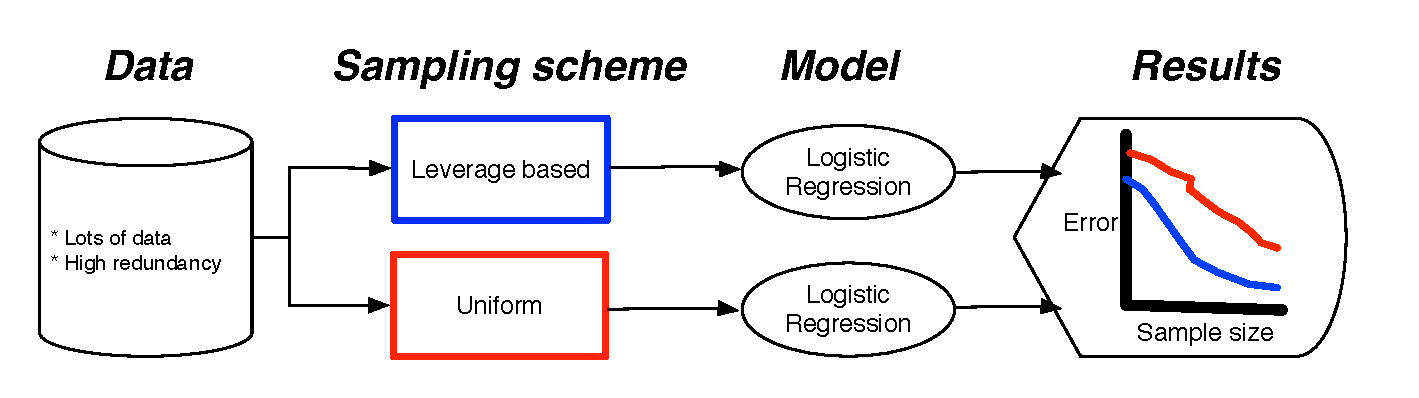
\includegraphics[width=\linewidth]{images/ThoughtModel}
\caption{The concept of leverage sampling}
\label{fig:concept}
\end{figure}
\section{Research Questions}
\begin{itemize}
	\item Can we validate the results for least-squares regression shown by Ma et al. \cite{Ma}
	\item Will a linear regression based sampling distribution improve our performance in classification?
	\item Can leverage based sampling be generalized and used for classification?
\end{itemize}

\section{Datasets}
These datasets are drawn from distributions defined in Ma et al. \cite{Ma} and characterized by
\begin{itemize}
	\item GA: Nearly uniform leverage-scores
	\item T3: Mildly non-uniform leverage-scores
	\item T1: Very non-uniform leverage-scores
\end{itemize}  
Samples from the three distributions are shown in {\bf Fig.~ \ref{fig:datasets}}

\begin{figure}[t]
\centering
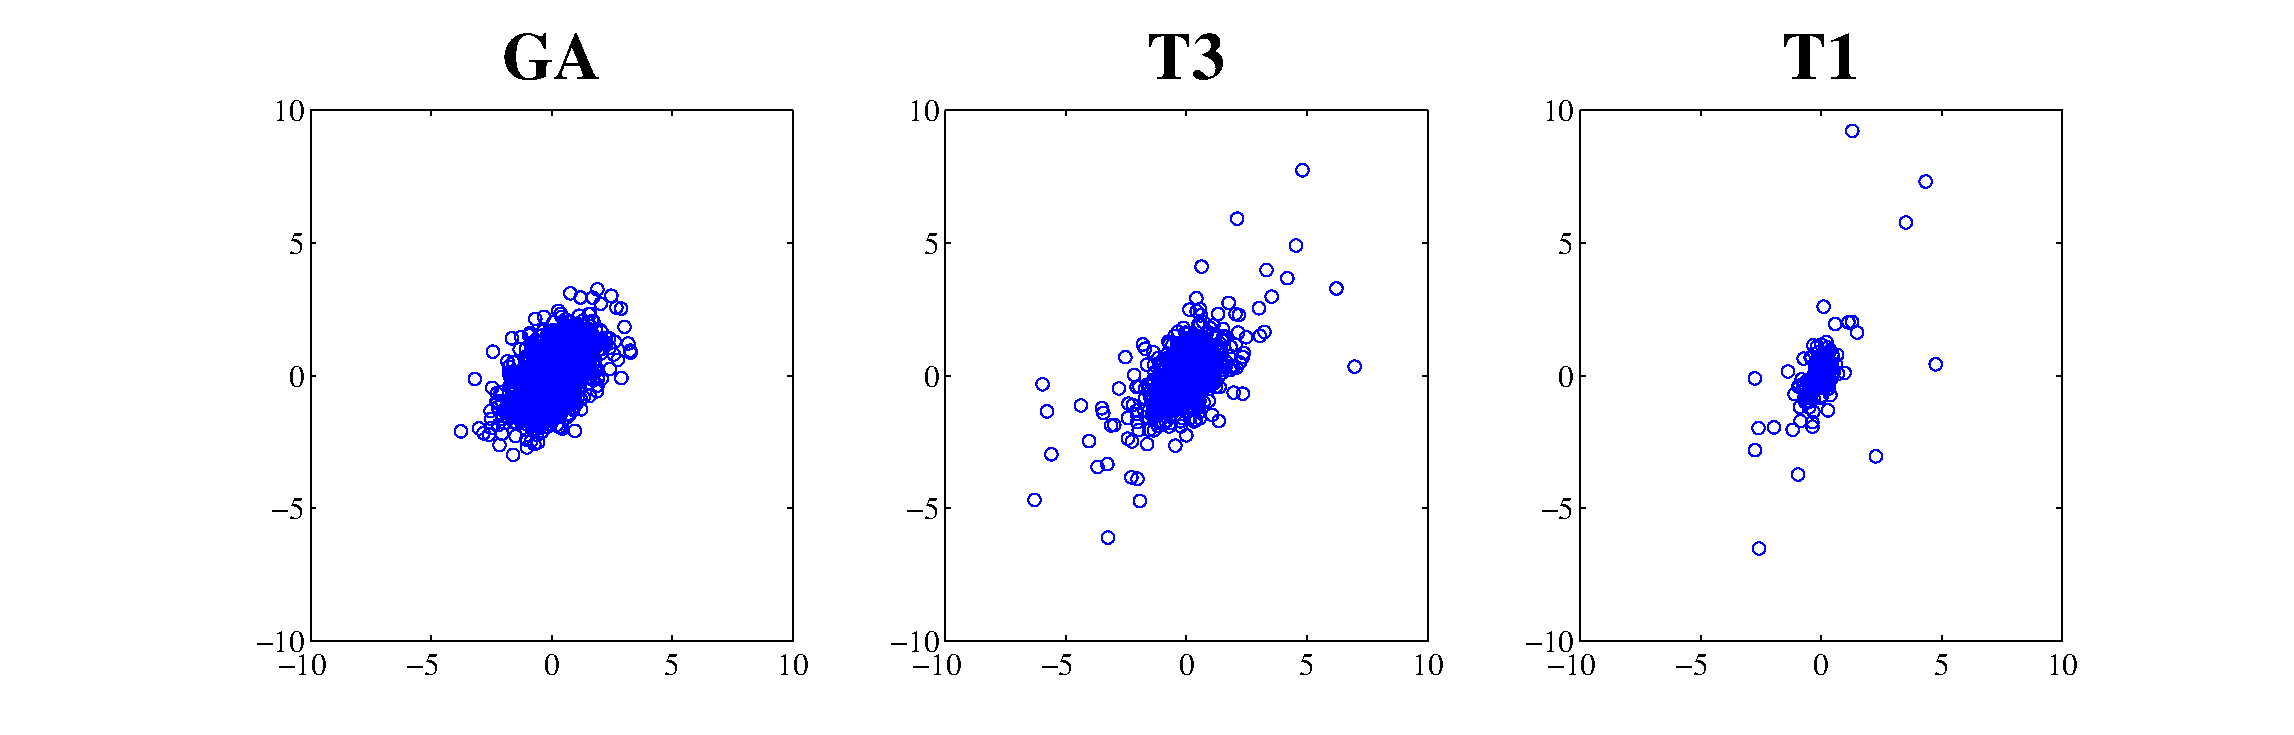
\includegraphics[width=\linewidth]{images/Data_distributions}
\caption{The three distributions considered standardized for comparison}
\label{fig:datasets}
\end{figure}
%

\section{Leveraging for least-squares regression}
When fitting a model, we know that some datapoints are more important that others, leveraging is based on the idea that we can determine the importance of a point beforehand and assign it a leverage-score to represent this.

\begin{enumerate}
\item A leverage-score is calculated for each datapoint.
\item These scores are normalized into a distribution $\pi$ to sample from.
\end{enumerate}

Ma. et al. \cite{Ma} use the leverage-scores for least-square regression defined as the diagonal elements of \eqref{eq:hdist}
\begin{equation}
\H = \X \left( \X^T \X \right)^{-1} \X^T
 \label{eq:hdist}
\end{equation}
This comes from the closed form expression for predictions which is linear in $y$
\begin{equation*}
	\hat{\y}_n = \X_n*\hat{\beta} \quad \text{where} \quad \hat{\beta} = \left( \X^T \X \right)^{-1} \X^T \y 
\end{equation*}

After normalizing this to a probability distribution we can sample  points that represent the structure better than a uniform sample. See {\bf Fig.~ \ref{fig:selection}}

\begin{figure}[t]
	\centering
    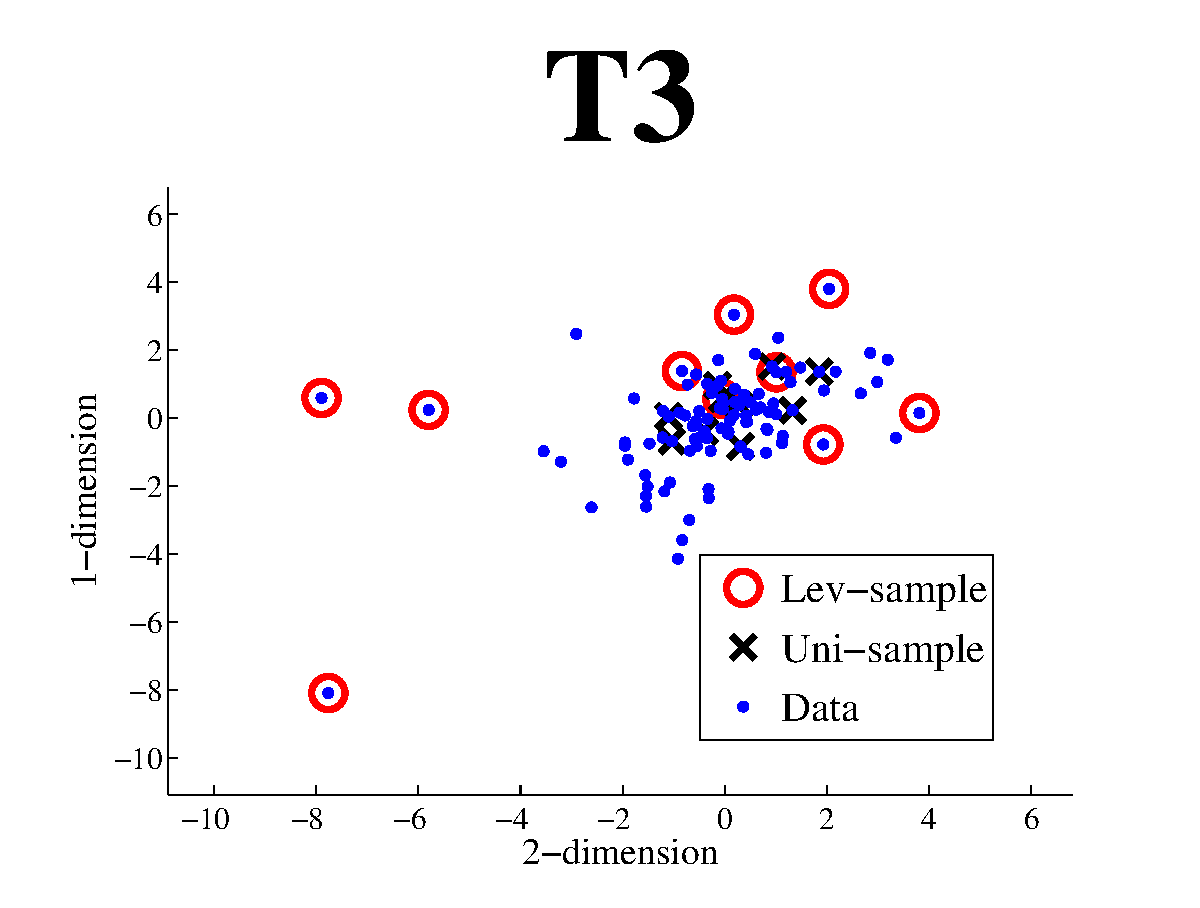
\includegraphics[width=.5\linewidth]{images/selection.eps}
    \caption{Comparison of sampling methods}
    \label{fig:selection}
\end{figure}


\section{Validation of previous results}
We have empirically tested and validated the results shown by Ma et al. \cite{Ma}. This is shown in {\bf Fig.~ \ref{fig:regression_results}}
\begin{figure}[!b]
\centering
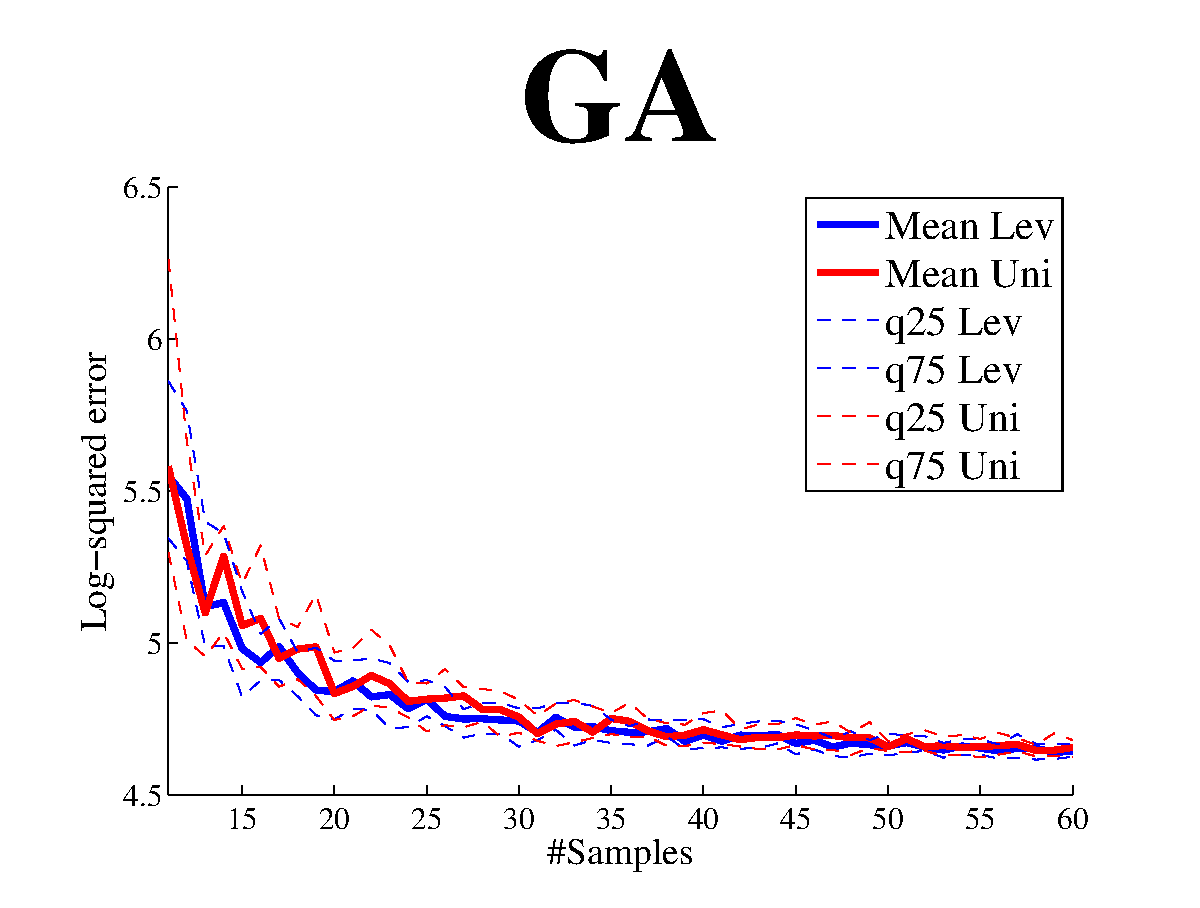
\includegraphics[width=.49\linewidth]{images/GALS.eps}
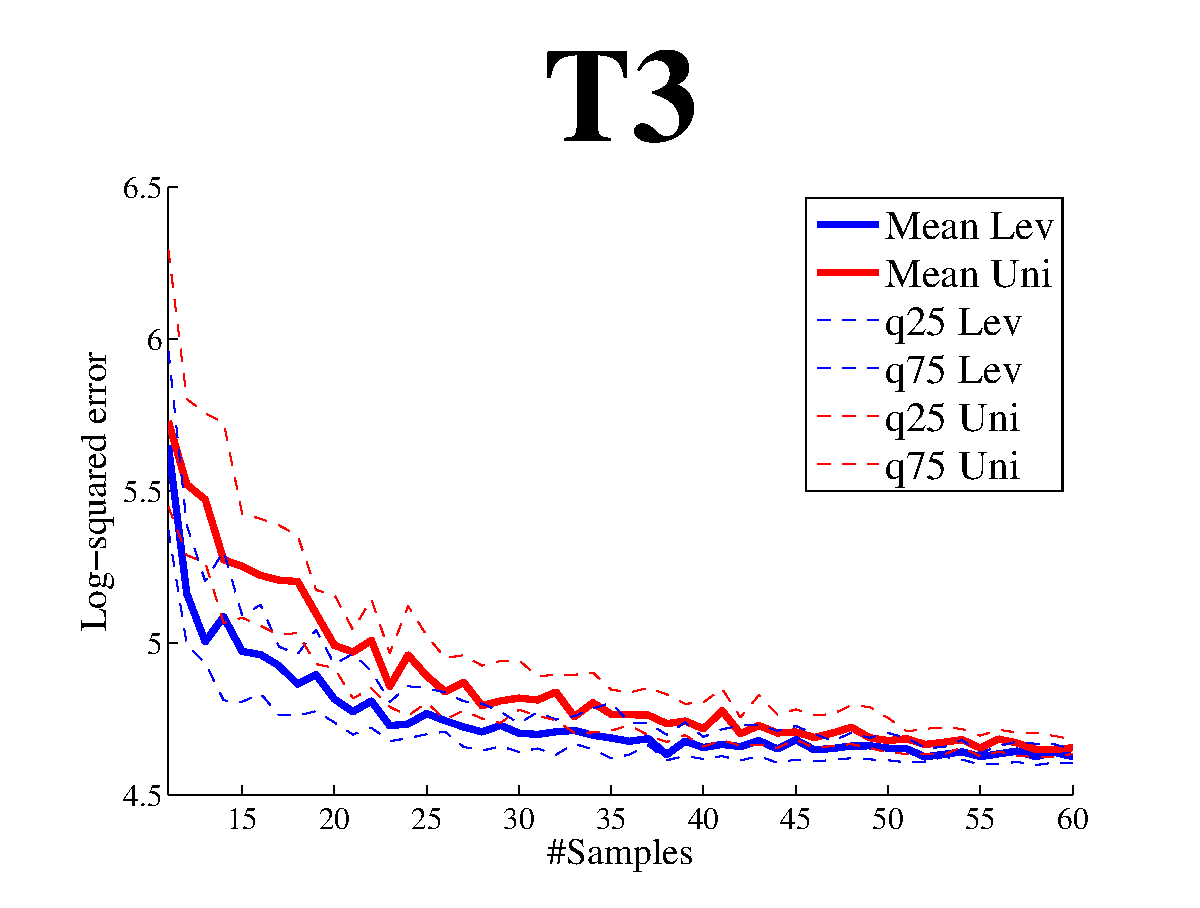
\includegraphics[width=.49\linewidth]{images/T3LS.eps}
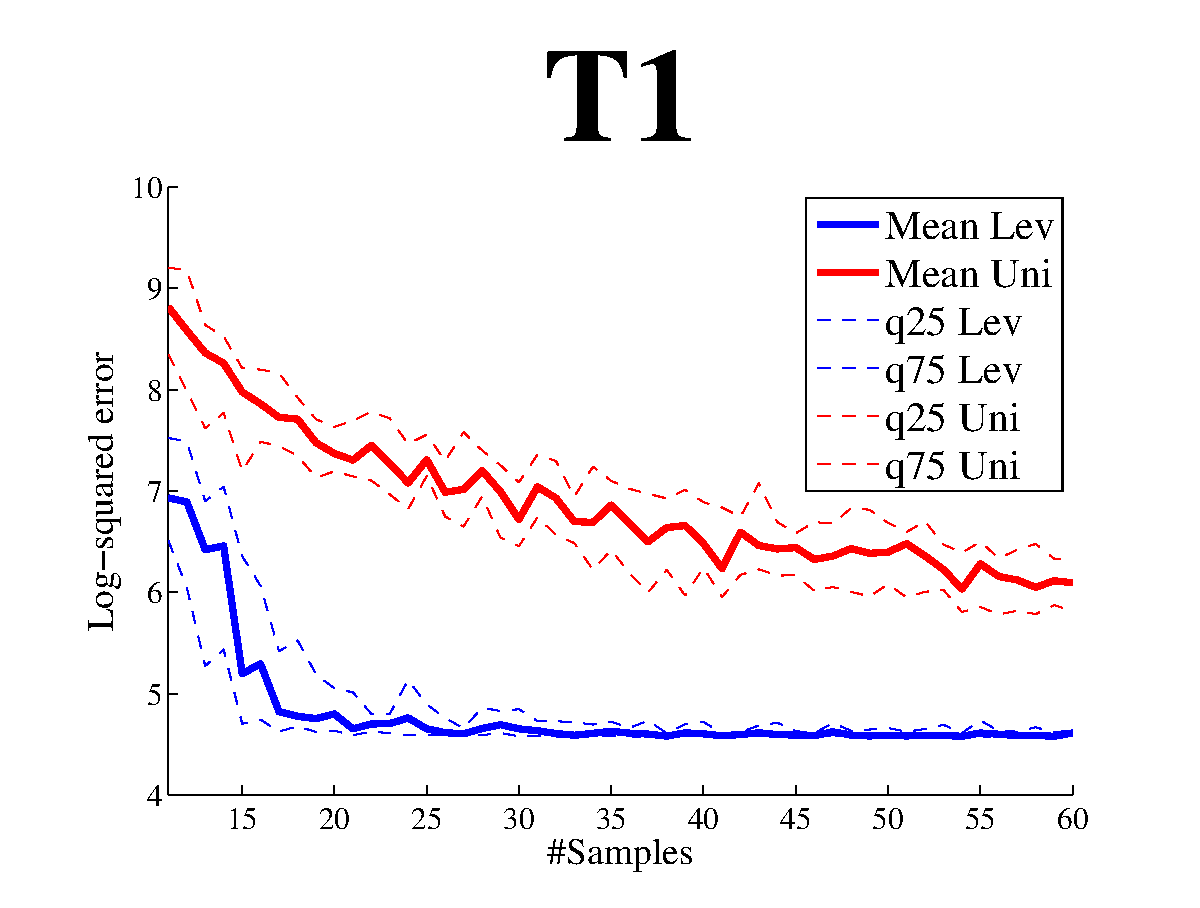
\includegraphics[width=.49\linewidth]{images/T1LS.eps}
\caption{Comparison of uniform {\bf\color{red}(red)} vs. leverage {\bf\color{blue}(blue)} based sampling schemes for least-squares regression. $N = 1000$, $d = 10$.}
\label{fig:regression_results}
\end{figure}

\begin{itemize}
\item GA: The leverage score are approximately uniform, and thus there is no significant difference between the two sampling schemes.
\item T3: Leveraging consistently provides slightly better results compared to uniform sampling.
\item T1: With \emph{very non-uniform} leverage-scores, leveraging clearly outperforms uniform sampling.
\end{itemize}

There results are consistent when varying $N$ and $d$, although the level of improvement varies.
%
\section{Datasets Binary Classification}
We define three datasets GA, T3 and T1, which resemble the ones from Ma et al. only for classification.

The data is generated by as for regression, but then split into two sets by adding a random unit vector scaled by the variance and a distance constant of 1.3. See Fig~\ref{fig:datasetsClass}.

\begin{figure}[t]
\centering
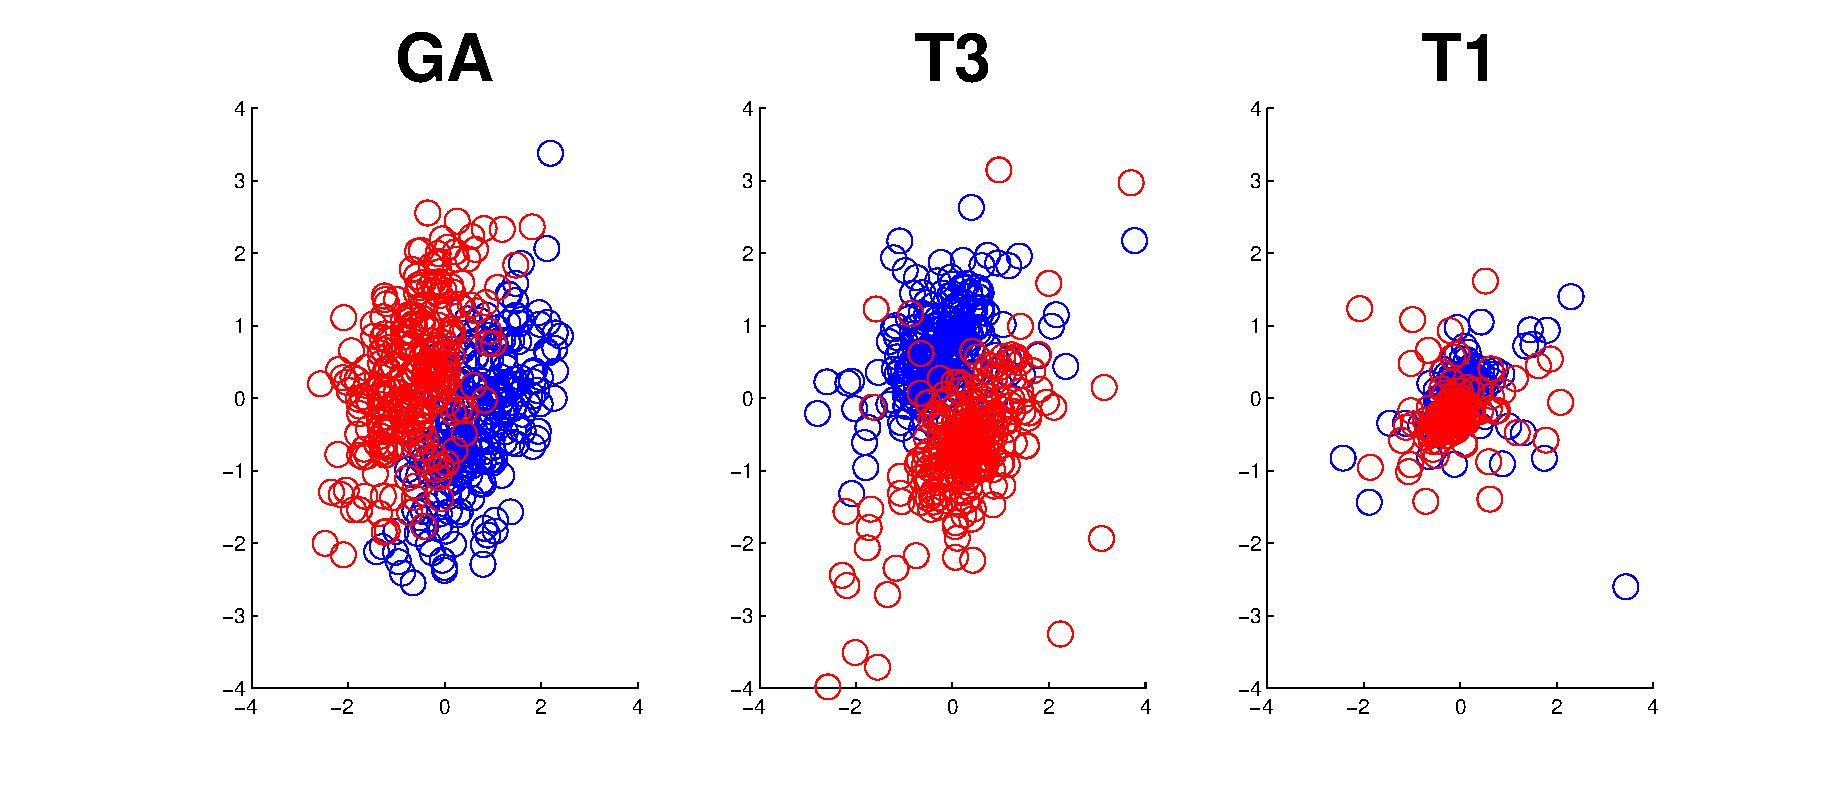
\includegraphics[width=\linewidth]{images/Data_distributionsClass}
\caption{The three distributions for binary classification standardized for comparison}
\label{fig:datasetsClass}
\end{figure}

\section{least-squares-based Distribution for Classification}

We sample from the same distribution \eqref{eq:hdist} as for least-squares regression. We use these samples to train a logistic regression model for binary classification, with equal class size.
 
  
\section{Test Results for least-squares-based sampling}
We compared the LS-distribution {\bf\color{blue}(blue)} to a uniform-distribution {\bf\color{red}(red)} in sampling for a logistic regression. The mean, 25th and 75th quantile are plotted. See {\bf Fig.~ \ref{fig:LS_class}}.
\begin{figure}[t]
\centering
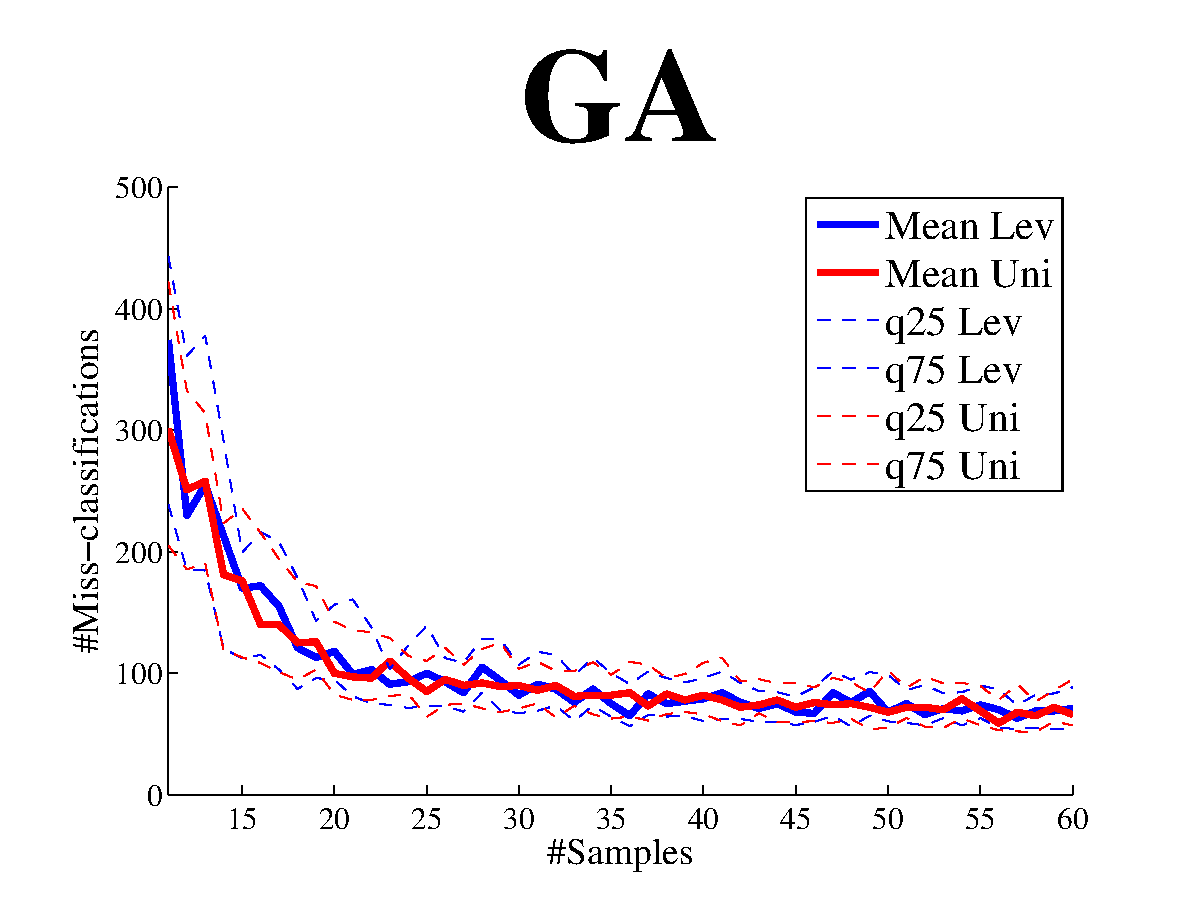
\includegraphics[width=.49\linewidth]{images/GA.eps}
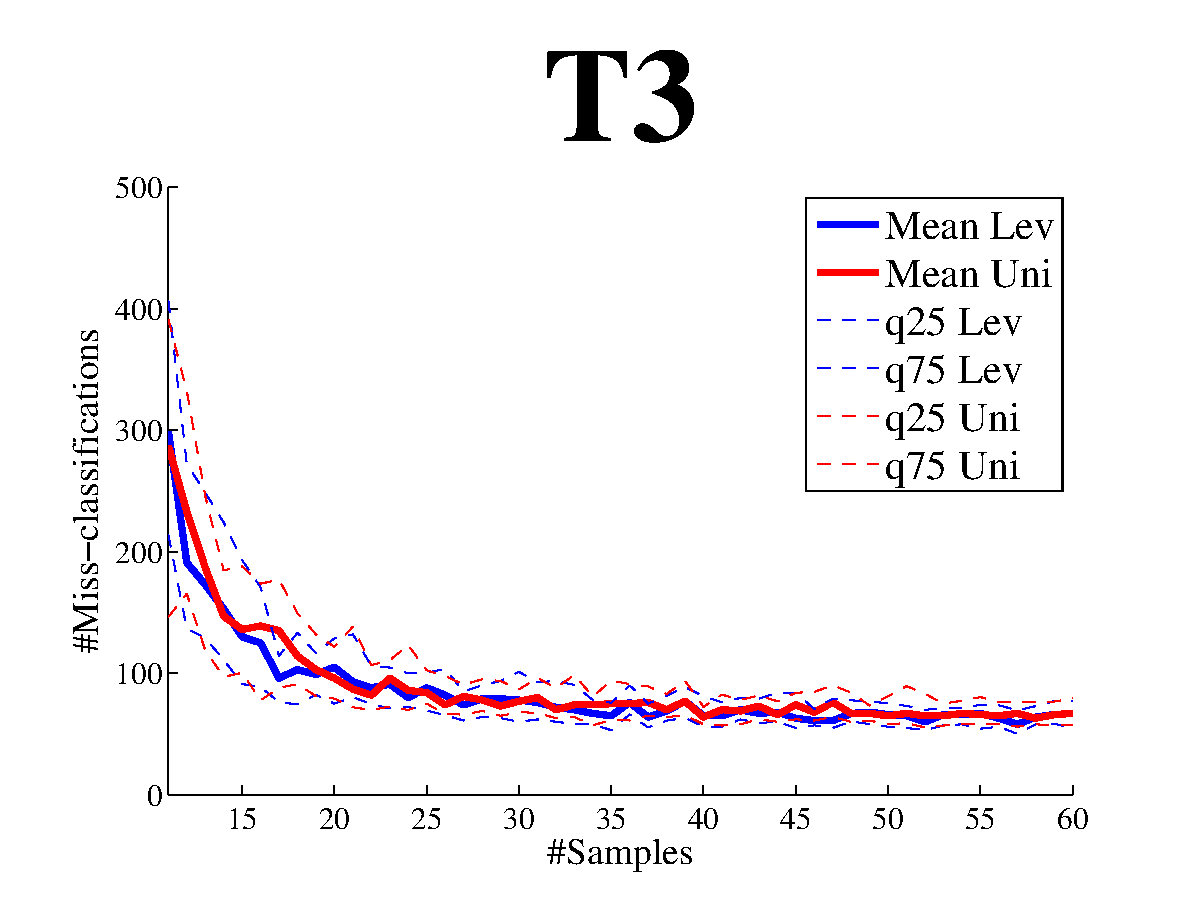
\includegraphics[width=.49\linewidth]{images/T3.eps}
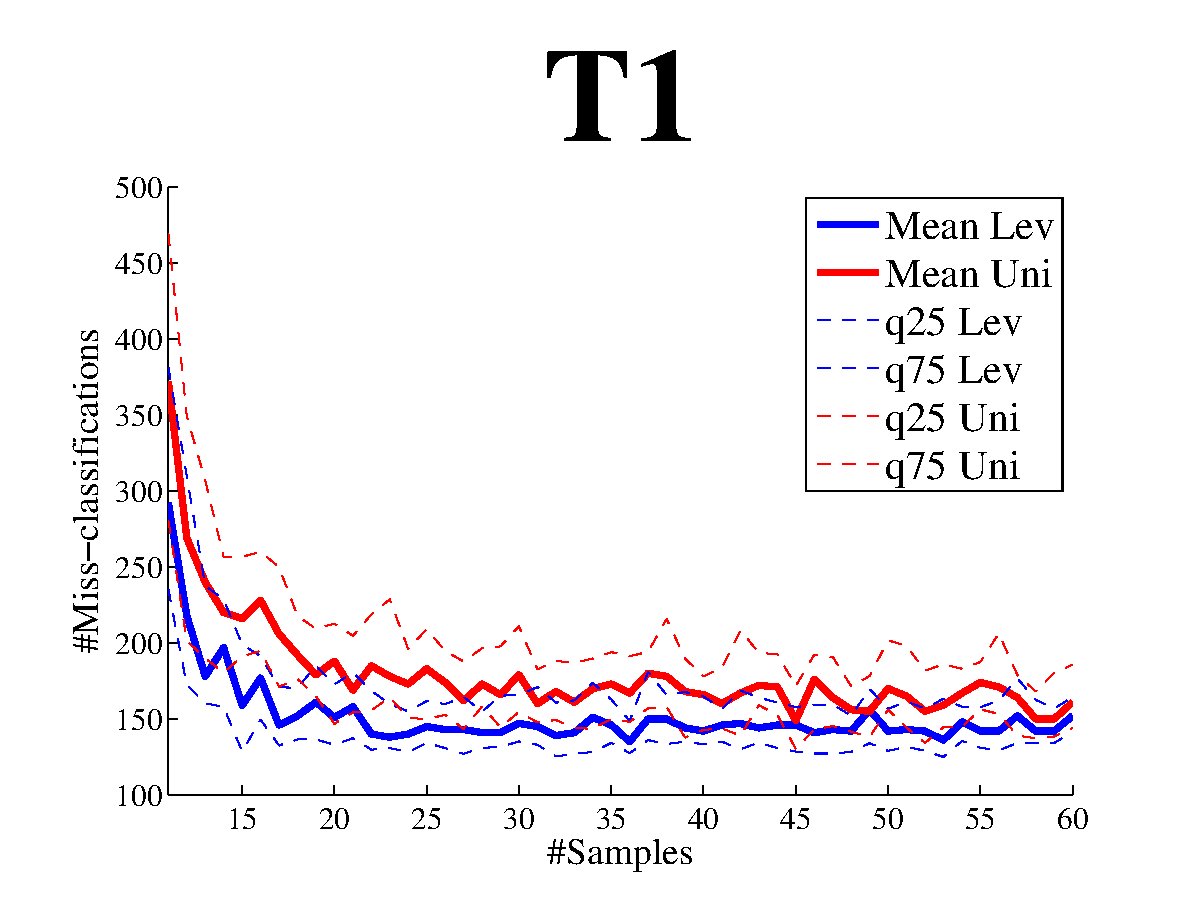
\includegraphics[width=.49\linewidth]{images/T1.eps}
\caption{Comparison of uniform {\bf\color{red}(red)} vs. leverage {\bf\color{blue}(blue)} based sampling schemes for classification. $N = 1000$, $d = 10$.}
\label{fig:LS_class}
\end{figure}	
\begin{itemize}
\item Sampling from the LS-distribution is no better that uniform on datasets of type GA and T3.
\item With very non-uniform leverage scores, T1, the LS-distribution slightly outperforms uniform sampling.
\end{itemize}
%It shows that a LS-distribution sample scheme, does not outperform a uniform-distribution for classification. 
The results shown are for dimension $p = 10$ and $N = 1000$ datapoints, but it is consistent when varying $p$ and $N$. \\
%
\section{Sensitivity Based Distribution}

We generalize the leverage scores to other models by seeing that they can be described as: 
	    \begin{equation}
	    \label{dyhatdy}
	    \frac{\delta \hat{\y}_n}{\delta \y_n} = Diag\left(H\right)
	    \end{equation}

Which we call the sensitivity of the model to a specific datapoint. For a general probabilistic discriminative model this requires the following:
    	\begin{equation}
    	 \hat{\y}_n = p(y|\bar{\x_n},\bar{\w}) \quad \bar{\w} \  \text{s.t.} \ \frac{\delta L}{\delta\bar{\w}}=0     	\label{optimum}
    	\end{equation}
Since \eqref{optimum} depends both directly and indirectly on $y$ we see that
    	\begin{equation}
    	\frac{\delta}{\delta \y} \frac{\delta \mathcal{L}}{\delta \w} = 0 
    	\Rightarrow
    	\frac{\delta^2 \mathcal{L}}{\delta \y \delta \bar{\w}} + \frac{\delta^2 \mathcal{L}}{\delta \bar{\w} \delta \bar{\w}^T} \frac{\delta \bar{\w}}{\delta \y}= 0
    	\end{equation}
    	
    	and from this we can get an expression for our leverage-score \eqref{dyhatdy}
    	
    	\begin{align}
    		\frac{\delta \hat{\y}_n}{\delta \y_n}&=\frac{\delta p(y|\bar{\x}_n,\bar{\w})}{\delta \bar{\w}^T} \frac{\delta \bar{\w}}{\delta \y} \nonumber \\
    		&= - \frac{\delta p(y|\bar{\x}_n,\bar{\w})}{\delta \bar{\w}^T} \left[ \frac{\delta^2 \mathcal{L}}{\delta \bar{\w} \delta \bar{\w}^T} \right]^{-1} \frac{\delta^2 \mathcal{L}}{\delta \y \delta \bar{\w}} \label{eq:sen}
    	\end{align}
    	
    	When using this model, initial weights are found by fitting a small uniform sample. This is expected outperform LS-based sampling since it introduces dependence on class information.
%

\section{Sensitivity for Logistic regression}

In the generalised sensitivity expression \eqref{eq:sen} we insert logistic regression and the log-likelihood function. Where we need the following expressions:
%Previously it is seen that the needed expressions are:

\begin{align*}
- \frac{\delta p(y|\bar{\x}_n,\bar{\w})}{\delta \bar{\w}^T}=&
X_n\frac{e^{-X*w_0^T}}{e^{-X*w_0^T}+1}\\
 \left[ \frac{\delta^2 \mathcal{L}}{\delta \bar{\w} \delta \bar{\w}^T} \right]^{-1}=&
 \sum_{n=1}^{N}  t_n X_n^T X_n \frac{e^{-X_n w_0^T}}{e^{-X_nw_0}+1}\\&+(1-t_n) \frac{X_n^T X_n}{e^{-X_nw_0}+1}\\
 \frac{\delta^2 \mathcal{L}}{\delta \y \delta \bar{\w}}=& \sum_{n=1}^{N} X_n
\end{align*}





\section{Test results for sensitivity based sampling}

\begin{figure}[t]
\centering
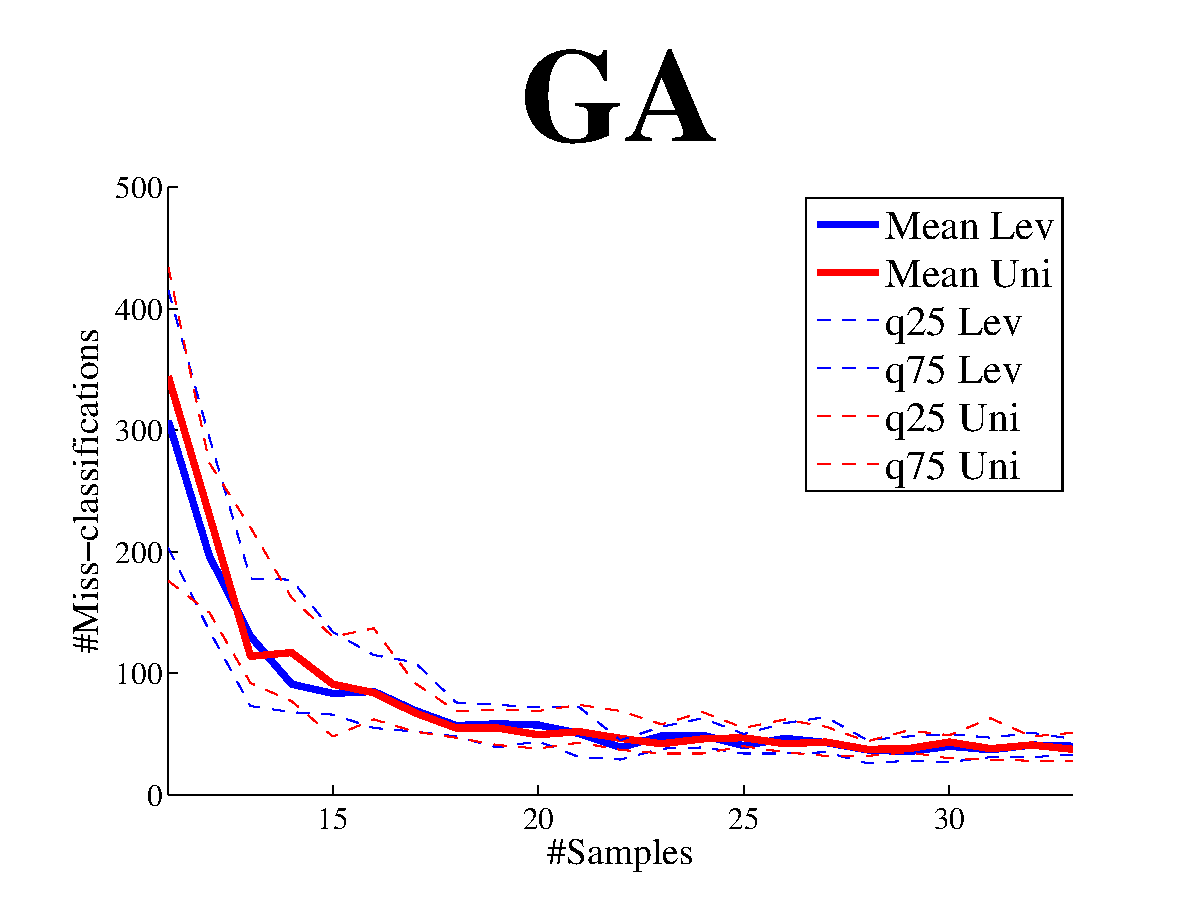
\includegraphics[width=.49\linewidth]{images/GAsen.eps}
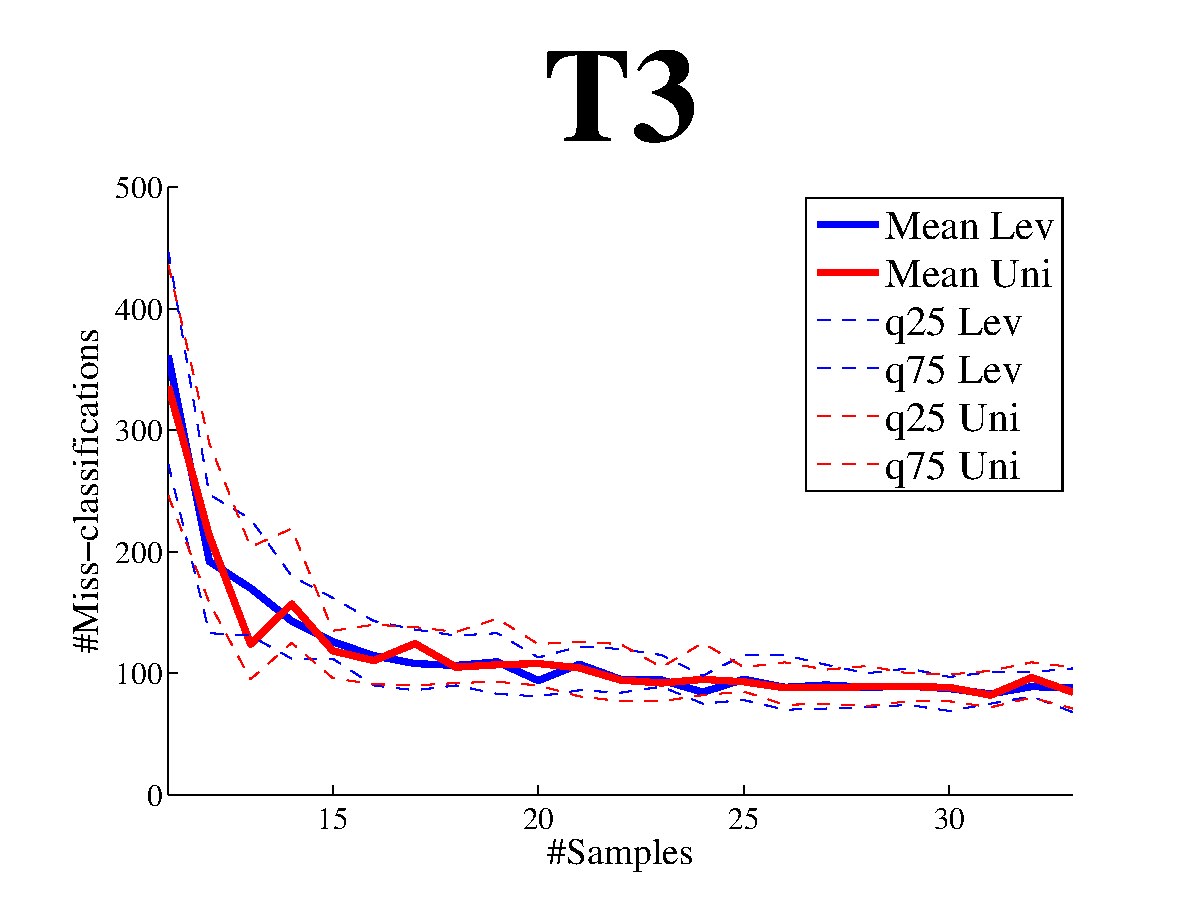
\includegraphics[width=.49\linewidth]{images/T3sen.eps}
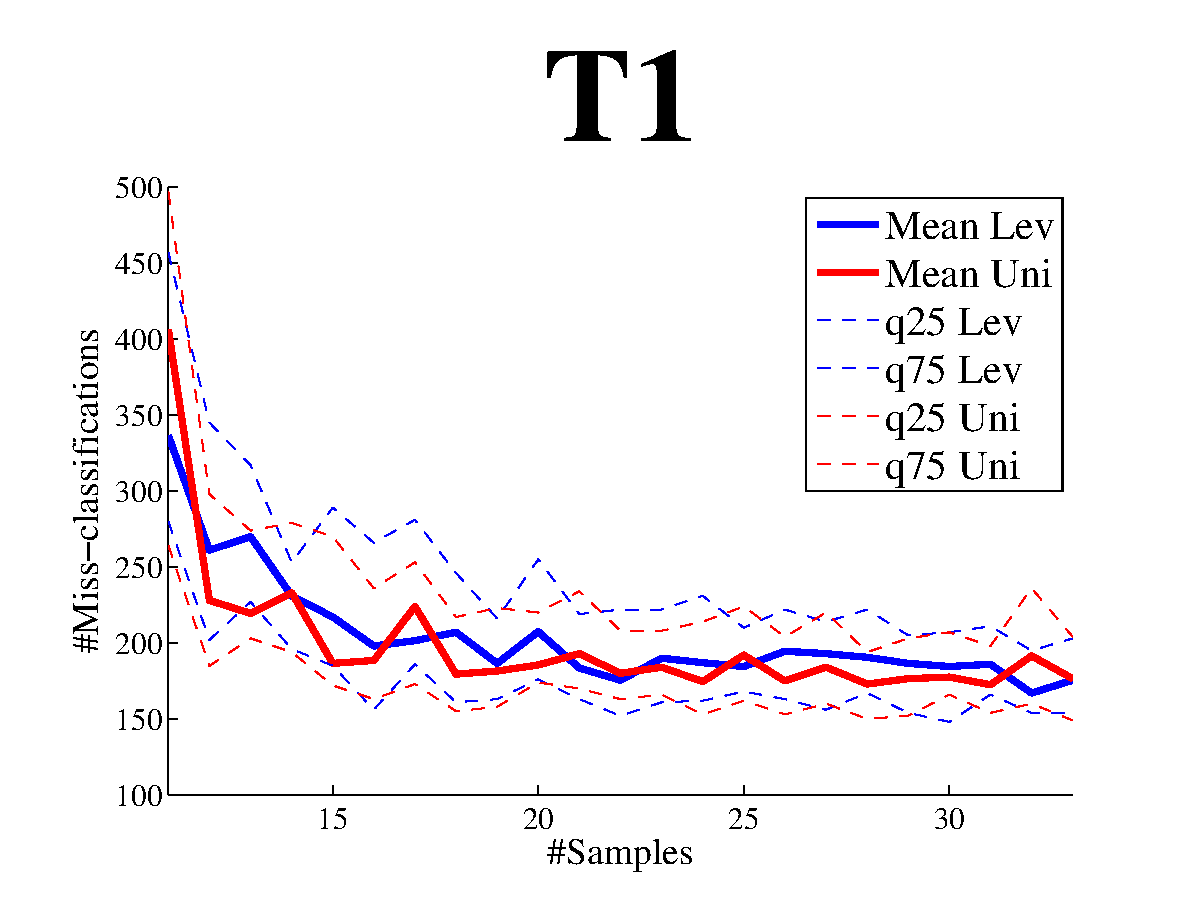
\includegraphics[width=.49\linewidth]{images/T1sen.eps}
\caption{Comparison of uniform {\bf\color{red}(red)} vs. sensitivity {\bf\color{blue}(blue)} based sampling schemes for logistic regression.}
\label{fig:SENS_class}
\end{figure}	

We see that the \emph{sensitivity based sampling} gives us a performance  equivalently to that of uniform sampling. Shown in {\bf Fig.~ \ref{fig:SENS_class}}
%
\section{Future work}
From our work several new question arise.
\begin{itemize}
\item How large show the initial sampling size be for sensitivity-based sampling?
\item Should the non-linear sensitivity based leverage scores be transformed? and how?
\item Should all points be sampled from the initial weights found, or should the process be iterative?
\end{itemize}
%
\section{Conclusion}
In the case of linear regression, leverage-based sampling provides a improvement over uniform sampling when the leverage-scores are mildly or very non-uniform.

Using the LS-based sampling for classification is slightly better with very non-uniform leverage-scores, T1 data.
%Using the LS-based sampling for classification shows no improvement on datasets \emph{GA} and \emph{T3}, but for \emph{T1} with very non-uniform leverage-scores, the approach is slightly better.

We have generalized the concept of leverage-based scores to classification with logistic regression and it has shown no improvements. However further analysis and tweaking might improved this approach.
%The LS-based leverage sampling gives no advantage over uniform sampling and generally performs worse. LS-distribution is based on what is important for linear regression, it does not have an advantage in finding important points for classification.


\bibliographystyle{IEEEbib}
\bibliography{./mlbib}

\end{document}
